%-------------------------
%device-revisited.tex
%(c) H.Buchmann FHNW 2018
%export TEXINPUTS=${HOME}/fhnw/edu/:${HOME}/fhnw/edu/tinL/config/latex:${HOME}/fhnw/edu/config//:
%-------------------------
\documentclass{beamer}
\usepackage{latex/beamer}
%---------------------
%local defines
%(c) H.Buchmann FHNW 2009
%$Id$
%---------------------
\newcommand{\target} {\beaglebone\xspace}
\newcommand{\targetS}{{\bf BBG}\xspace}
\newcommand{\host}   {{\em Host}\xspace}
\newcommand{\targetroot} {{\bf target-root}\xspace}
\newcommand{\kernel} {{\bf kernel}\xspace}
\renewcommand{\c}{{\bf C}\xspace}
\newcommand{\cpp}{{\bf C++}\xspace}
\newcommand{\posix}{{\bf POSIX}\xspace}

\usepackage{svg}
\usepackage[absolute]{textpos}
\setlength{\TPHorizModule}{1mm}
\setlength{\TPVertModule}{1mm}

\begin{document}


\newcommand{\ksp}{{\em kernel-space}\xspace}
\newcommand{\usp}{{\em user-space}\xspace}

\title[Kernel-User]{Kernelspace-userspace\\call-back}

\frame{\titlepage}

\begin{frame}{Outline}
 \begin{itemize}
  \item The Big Picture
  \begin{itemize}
   \item call-back, notification
  \end{itemize}
  \item \linux KernelSpace-UserSpace am Beispiel \targetS
  \begin{itemize}
   \item \cod{hotplug}
   \item \cod{socket NETLINK KOBJECT UEVENT}
  \end{itemize}
  \remark{gilt für alle \linux}
 \end{itemize}
\end{frame}

\section{The Big Picture}
\begin{frame}{Typisches Szenario}{USB-Stick einstecken}
 \begin{enumerate}
  \item Hardware Interupt
  \item Kernel behandelt den Interrupt
  \item Informiert (notifiziert) {\em user} 
  \begin{itemize}
   \item device name: \cod{/dev/sdXY}
  \end{itemize}
  \item {\em user}  montiert Filesystem 
  \begin{itemize}
   \item \cod{mount /dev/sdXY /mount-path}
  \end{itemize}
 \end{enumerate}
\end{frame}

\begin{frame}{KernelSpace-UserSpace}
\begin{center}
 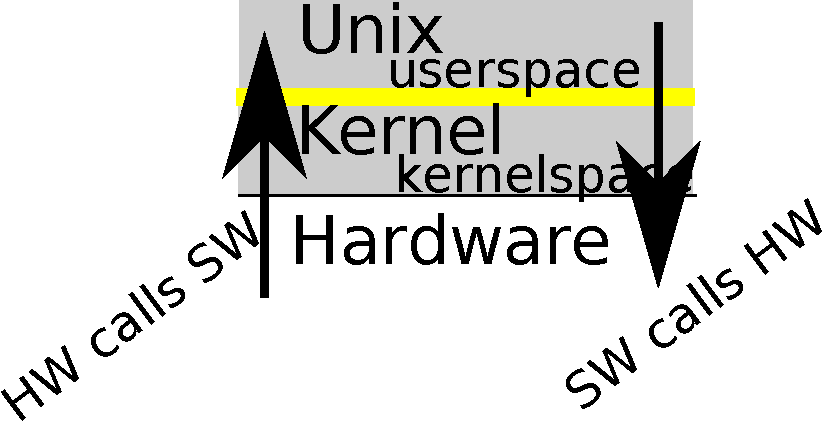
\includegraphics[width=0.875\textwidth]{hw-calls-sw.pdf}
\end{center}
\end{frame}

\begin{frame}{SW calls HW}{UserSpace $to$ KernelSpace}
 \begin{itemize}
  \item \cod{date}
  \begin{itemize}
   \item Klassisch der "normale"{} Fall
  \end{itemize}
 \end{itemize}
\end{frame}

\begin{frame}{HW calls SW}{KernelSpace $to$ UserSpace}
 \begin{itemize}
  \item Hardware bemerkt etwas \cod{USB-Stick}
  \item Informiert den {\em user} 
  \begin{itemize}
   \item Klassisch der "abnormale"{} ungeliebte Fall
  \end{itemize}
 \end{itemize}
\end{frame}

\begin{frame}{Informieren}{verschiedene Wörter}
 \begin{itemize}
  \item Notifizieren {\em notify} 
  \item Zurückrufen {\em call-back}
  \item hotplug
 \end{itemize}
\end{frame}

\section{\linux am Beispiel \targetS}
\subsection{hotplug}

\begin{frame}{Hotplug}{/proc/sys/kernel/hotplug}
 \begin{itemize}
  \item Kernel: {\em kernel-space} entdeckt ein neues Gerät
  \item Informiert (notify) User user-space: neues Gerät
  \begin{itemize}
   \item call-back: \cod{/proc/sys/kernel/hotplug} 
   \begin{itemize}
    \item enthält Name eines {\em user-space} executables
   \end{itemize}
  \end{itemize}
 \end{itemize}
 \remark{Kernel muss für {\em hotplug} konfiguriert sein}
\end{frame}

\begin{frame}{Hotplug Beispiel}
 \begin{itemize}
  \item File: \cod{hotplug.sh}
  \item executable 
  \begin{itemize}
   \item \cod{chmod a+x hotplug.sh}
  \end{itemize}
  \item Register
  \begin{itemize}
   \item \cod{echo {\em absolute-path-to-hotplug.sh} > /proc/sys/kernel/hotplug}
  \end{itemize}
 \end{itemize}
\end{frame}

\subsection{Socket}

\begin{frame}{Socket}{Alles ist ein Socket}
 \begin{itemize}
  \item Endpunkt einer Verbindung (Buchse)
  \item verschiedene Typen
  \begin{itemize}
   \item Internet
   \item Verbindung vom kernel
   \item \cod{netstat}
  \end{itemize}
 \end{itemize}
\end{frame}

\begin{frame}{Socket}{KerneSpace-UserSpace}
 \begin{itemize}
  \item Kernel: entdeckt neues Gerät ({\em device})
  \item Kernel: sendet Daten an einen Socket
  \item User: liest die Daten
 \end{itemize}
\end{frame}

\begin{frame}{Beispiel}
\begin{itemize}
 \item C:
 \begin{itemize}
  \item \cod{uevent-userspace.c}
  \item \cod{split.c} für die schöne Ausgabe
 \end{itemize}
 \item C++
 \begin{itemize}
  \item \cod{uevent.h/cc} das Modul
  \item \cod{uevent-demo.cc} eine einfache Anwendung
 \end{itemize}
\end{itemize}
\end{frame}

\end{document}
